\documentclass[a4paper,11pt]{jsarticle}

\usepackage{amsmath,amsfonts,amssymb}

\usepackage{bm}
\usepackage[dvipdfmx]{graphicx}
\usepackage{multirow}
\usepackage[hang,small,bf]{caption}
\usepackage[subrefformat=parens]{subcaption}
\captionsetup{compatibility=false}
\usepackage{url}

\begin{document}

\title{Advanced Machine Learning Midterm Assignment}
\author{情報工学系 19B39038 三嶋 隆史}
\date{\today}

\maketitle

\section*{問題 1}
\subsection*{1, 2}
\hbox{実装したソースコードを以下のリンクに示す.}{https://github.com/Mishima-Ryuji/aml2022/blob/master/src/problem.md}

\subsection*{3}
ニュートン法を実行した結果を青,勾配降下法を実行した結果を赤として,以下の図に示す.結果からわかるように,ニュートン法は初期で収束していることが確認できる.
\begin{center}
    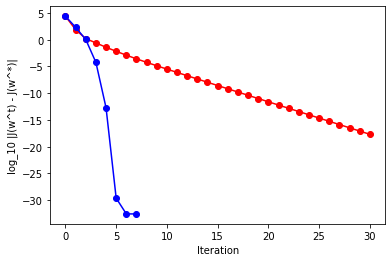
\includegraphics[width=5cm]{../src/output_7_1.png} \\
\end{center}

\subsection*{4}
パラメータ$w$の時に,データ$\bm x$が$y_i$に分類される確率$p(y|\bm x, \bm w)$を以下のように定める.
$$
    p(y_i|\bm x, \bm w) = \frac{\exp(\bm{w}_y^T\bm{x})}{\sum_{c=1}^{C} \exp(\bm{w}_c^T\bm{x})}
$$
ここで,データ$\bm x$に対する損失関数$l(f(\bm x), y)$を以下のように定める.
$$
    l(f(\bm x), y) = -\bm{w}_y^T \bm x + \ln \left(\sum_{c=1}^C \exp(\bm{w}_c^T \bm x) \right)
$$
次に$\nabla_{\bm{w}_y} l$および$\nabla_{\bm{w}_y}^2 l$を計算する.
$$
    \nabla_{\bm{w}_y} l = - \bm x +
    \frac{\exp(\bm{w}_y^T \bm x)}{\sum_{i = 1}^{C} \exp(\bm w_c^T \bm x)} \bm x
$$
$$
    \nabla_{\bm{w}_y}^2 l =
    \frac{\sum_{i = 1, c \neq y}^{C} \exp(\bm w_y^T \bm x) \exp(\bm w_c^T \bm x)}{ \left\{ \sum_{i = 1}^{C} \exp(\bm w_c^T \bm x) \right\}^2 }\bm{x}\bm x^T
$$
これらを使って,勾配降下法とニュートン法を実装する.実装を完了できませんでした.

\section*{問題 9}
\subsection*{1}
この問題は以下のように$\max$と平方根を含まない形に変換できる.
\begin{align*}
    \mathrm{Minimize:}    & \quad z                                           \\
    \mathrm{Subject\ to:} & \quad \forall i , (x_i - x)^2 + (y_i - y)^2 \le z \\
                          & \quad z \geq 0
\end{align*}
ここで,ラグランジュ緩和問題を求めると,
\begin{align*}
    \mathrm{Minimize:}    & \quad z - \sum_{i=1}^{n} \alpha_i \left\{
    z- (x_i - x)^2 - (y_i - y)^2 \right\}                                                                       \\
                          & \quad = \left(1 - \sum_{i=1}^{n}\alpha_i \right)z + \sum_{i=1}^{n} \alpha_i \left\{
    (x_i - x)^2 + (y_i - y)^2 \right\}
    \\
    \mathrm{Subject\ to:} & \quad z \geq 0                                                                      \\
                          & \quad \forall i , \alpha_i \geq 0
\end{align*}
となるから,ここから双対問題に変換すると,
\begin{align*}
    \mathrm{Maximize:}    & \quad \sum_{i=1}^{n} \alpha_i \left\{
    (x_i - x)^2 + (y_i - y)^2 \right\}                            \\
    \mathrm{Subject\ to:} & \quad  \sum_{i=1}^{n}\alpha_i  \leq 1 \\
                          & \quad \forall i , \alpha_i \geq 0
\end{align*}
が得られる.

\section*{問題 6}
$f(\hat{\bm w}) -f(\bm w^*) \le \epsilon $となる$T$を求めるためには,$f(\bm{w}^{(T)}) -f(\bm w^*) \le \epsilon $となる最も小さい$T=T^*$を見つければ良い.$T^*$について以下の式が成り立つ.
\begin{align*}
    f(\bm{w}^{(0)}) - f(\bm w^*) & = \left| f(\bm{w}^{(0)}) - f(\bm w^*) \right|                                                                                       \\
                                 & \le \sum_{i = 0}^{T^\ast - 1} \left| f(\bm{w}^{(i)}) - f(\bm{w}^{(i+1)}) \right| + \left| f(\bm{w}^{(T^\ast)}) - f(\bm w^*) \right| \\
                                 & \le \sum_{i = 0}^{T^\ast - 1} \left| f(\bm{w}^{(i)}) - f(\bm{w}^{(i+1)}) \right| + \epsilon                                         \\
                                 & \le \sum_{i = 0}^{T^\ast - 1} L \left\lVert \bm{w}^{(i)} - \bm{w}^{(i+1)} \right\lVert + \epsilon                                   \\
                                 & \le \sum_{i = 0}^{T^\ast - 1} \eta L \left\lVert \nabla f|_{\bm w = \bm{w}^{(t)}} \right\lVert + \epsilon                           \\
                                 & \le \eta L T^\ast \max_{0 \le t < T^\ast } \left\lVert \nabla f|_{\bm w = w^{(t)}} \right\lVert + \epsilon                          \\
                                 & \le \frac{\epsilon}{L} \max_{0 \le t < T^\ast } \left\lVert \nabla f|_{\bm w = w^{(t)}} \right\lVert + \epsilon
\end{align*}
よって,
\begin{align*}
    T^\ast \ge \frac{L(f(\bm{w}^{(0)}) - f(\bm w^*) - \epsilon)}{\epsilon \max_{0 \le t < T^\ast } \left\lVert \nabla f|_{\bm w = w^{(t)}} \right\lVert}
\end{align*}
\end{document}
